% Suggested LaTeX figure inclusion blocks. Requires graphicx (and booktabs for tables).
% Paths are relative to the report_assets_final/ directory.

\begin{figure}[htbp]
  \centering
  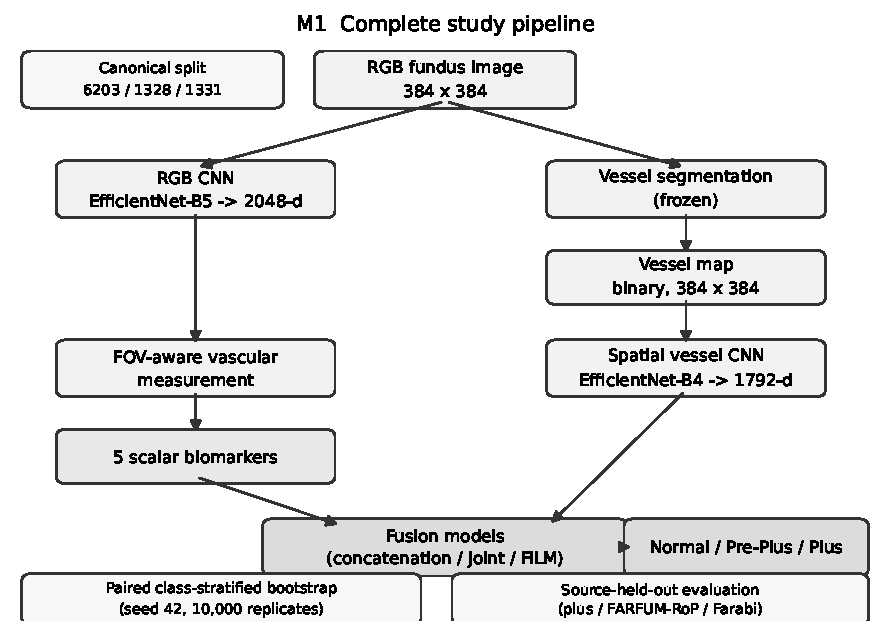
\includegraphics[width=\linewidth]{figures/methods/M1_complete_pipeline.pdf}
  \caption{Complete study pipeline. See captions/captions\_en.md (Figure M1) for the full caption, abbreviations, statistical test, sample size and any restricted-evaluation note.}
  \label{fig:pipeline}
\end{figure}

\begin{figure}[htbp]
  \centering
  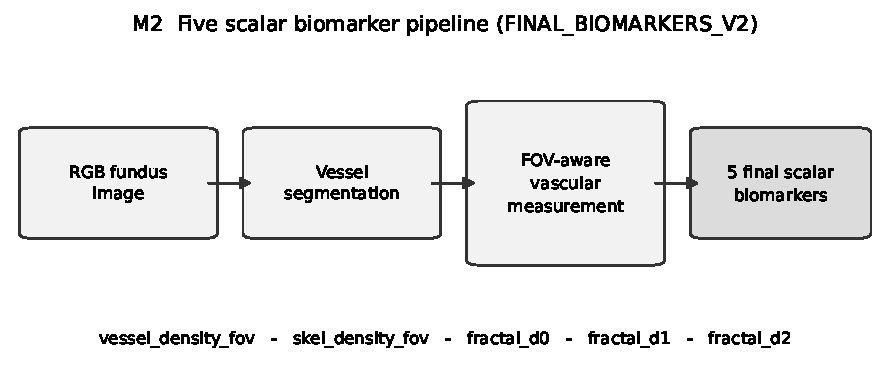
\includegraphics[width=\linewidth]{figures/methods/M2_biomarker_pipeline.pdf}
  \caption{Five scalar biomarker pipeline. See captions/captions\_en.md (Figure M2) for the full caption, abbreviations, statistical test, sample size and any restricted-evaluation note.}
  \label{fig:biomarkerpipeline}
\end{figure}

\begin{figure}[htbp]
  \centering
  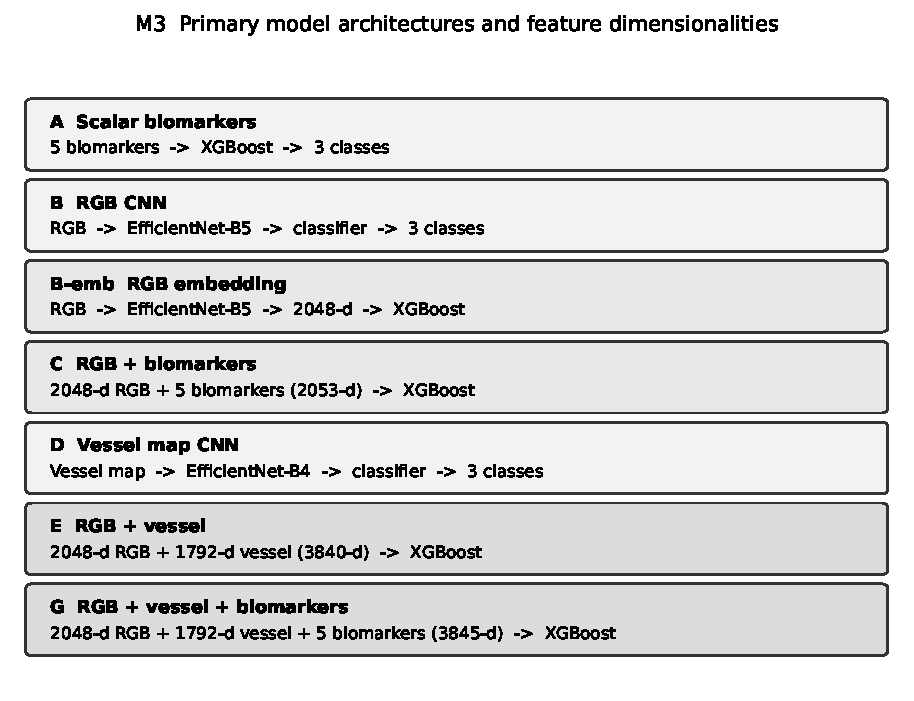
\includegraphics[width=\linewidth]{figures/methods/M3_model_architectures.pdf}
  \caption{Primary model architectures. See captions/captions\_en.md (Figure M3) for the full caption, abbreviations, statistical test, sample size and any restricted-evaluation note.}
  \label{fig:architectures}
\end{figure}

\begin{figure}[htbp]
  \centering
  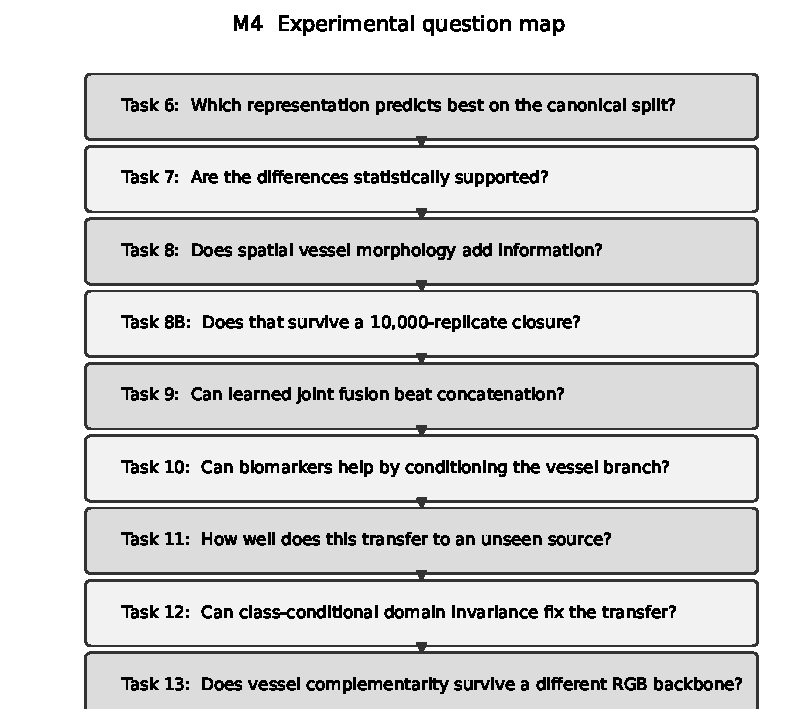
\includegraphics[width=\linewidth]{figures/methods/M4_experimental_question_map.pdf}
  \caption{Experimental question map. See captions/captions\_en.md (Figure M4) for the full caption, abbreviations, statistical test, sample size and any restricted-evaluation note.}
  \label{fig:questionmap}
\end{figure}

\begin{figure}[htbp]
  \centering
  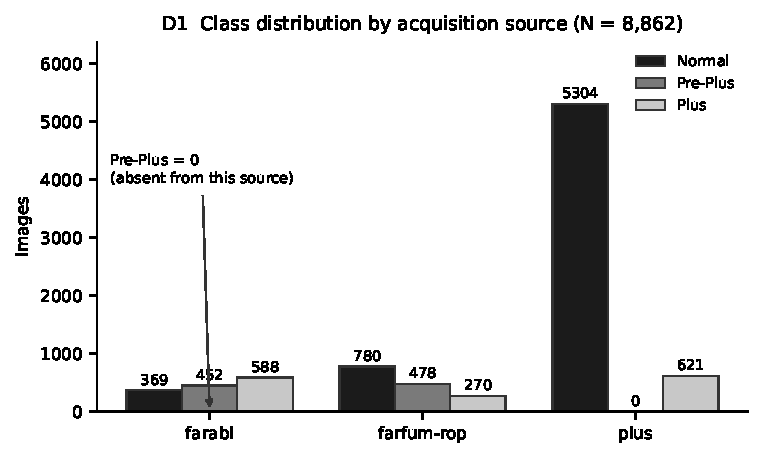
\includegraphics[width=\linewidth]{figures/main/D1_source_class_distribution.pdf}
  \caption{Class distribution by acquisition source. See captions/captions\_en.md (Figure D1) for the full caption, abbreviations, statistical test, sample size and any restricted-evaluation note.}
  \label{fig:sourceclass}
\end{figure}

\begin{figure}[htbp]
  \centering
  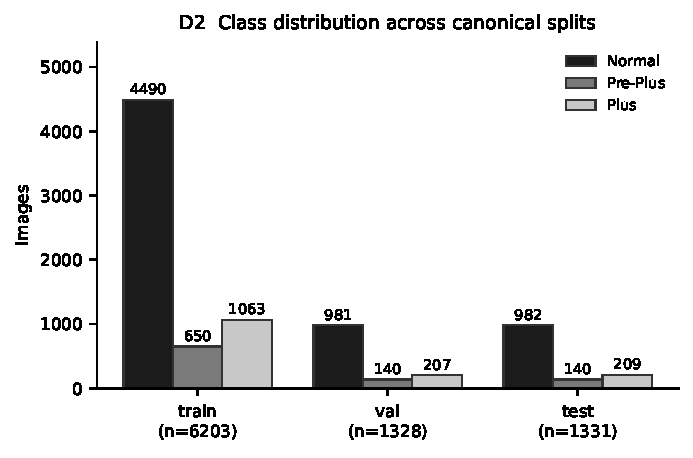
\includegraphics[width=\linewidth]{figures/main/D2_split_class_distribution.pdf}
  \caption{Class distribution across canonical splits. See captions/captions\_en.md (Figure D2) for the full caption, abbreviations, statistical test, sample size and any restricted-evaluation note.}
  \label{fig:splitclass}
\end{figure}

\begin{figure}[htbp]
  \centering
  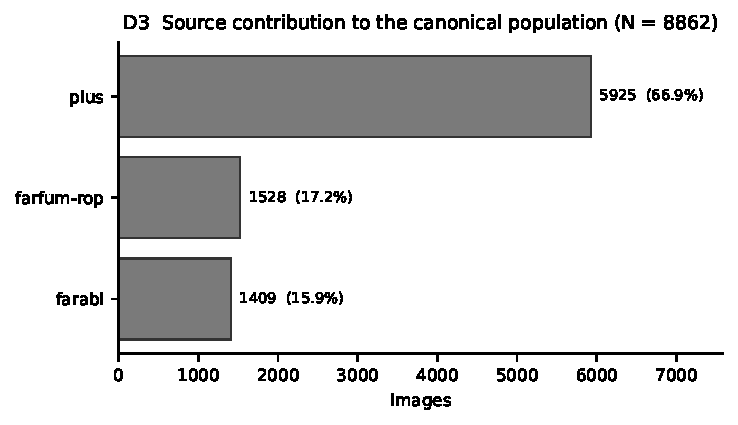
\includegraphics[width=\linewidth]{figures/main/D3_source_population.pdf}
  \caption{Source contribution to the canonical population. See captions/captions\_en.md (Figure D3) for the full caption, abbreviations, statistical test, sample size and any restricted-evaluation note.}
  \label{fig:sourcepopulation}
\end{figure}

\begin{figure}[htbp]
  \centering
  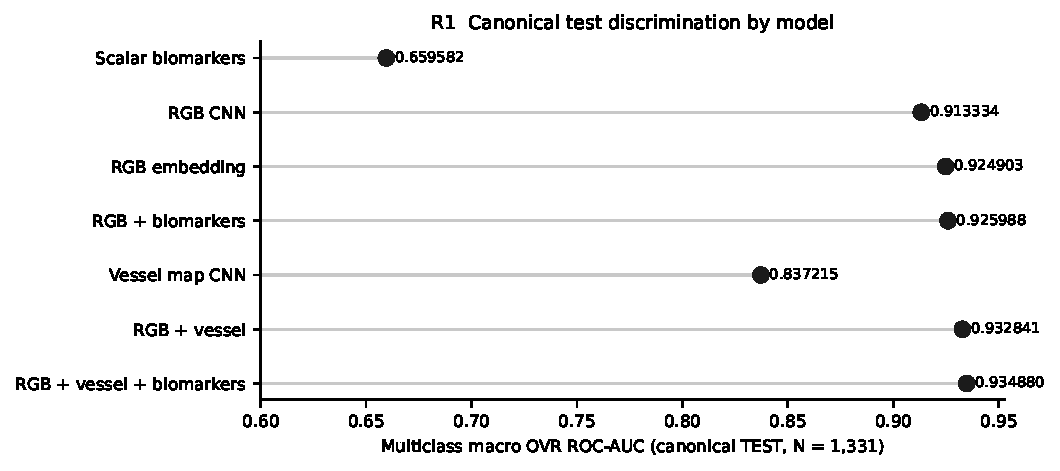
\includegraphics[width=\linewidth]{figures/main/R1_model_auc_comparison.pdf}
  \caption{Canonical test discrimination by model. See captions/captions\_en.md (Figure R1) for the full caption, abbreviations, statistical test, sample size and any restricted-evaluation note.}
  \label{fig:modelauc}
\end{figure}

\begin{figure}[htbp]
  \centering
  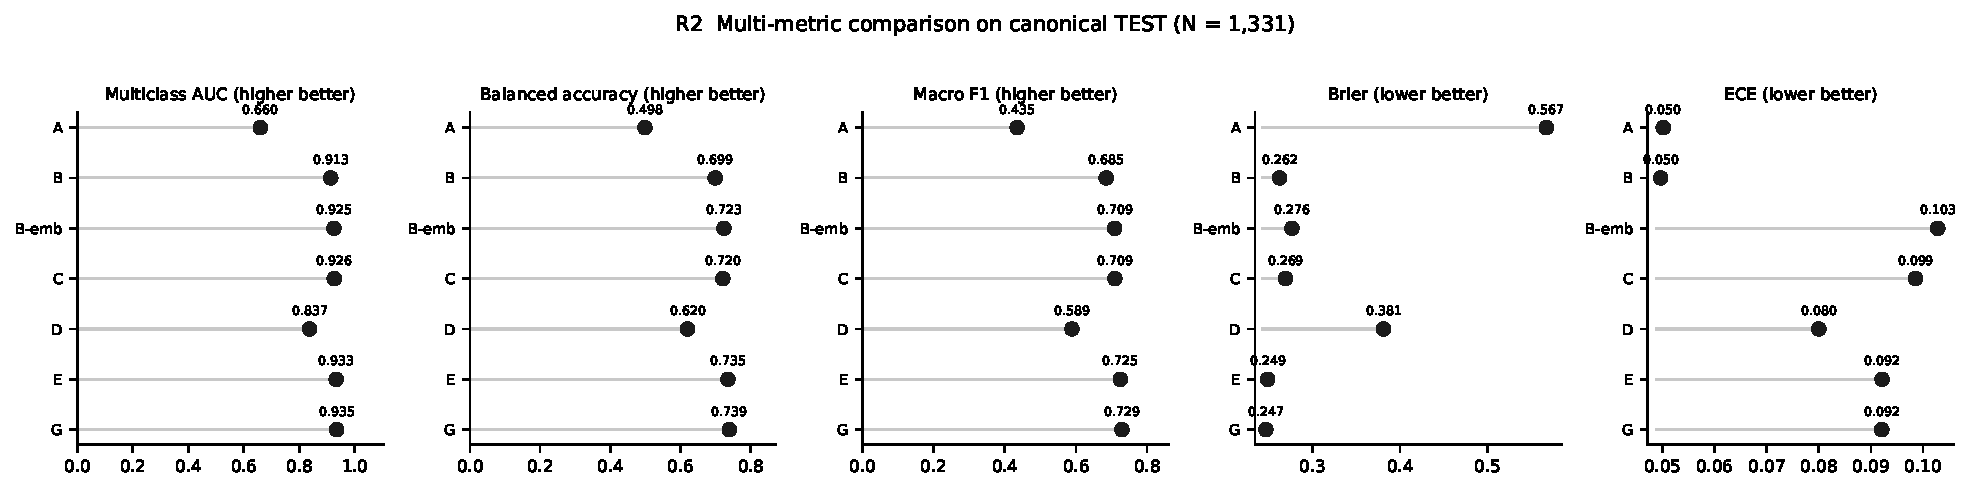
\includegraphics[width=\linewidth]{figures/main/R2_model_metric_panels.pdf}
  \caption{Multi-metric model comparison. See captions/captions\_en.md (Figure R2) for the full caption, abbreviations, statistical test, sample size and any restricted-evaluation note.}
  \label{fig:metricpanels}
\end{figure}

\begin{figure}[htbp]
  \centering
  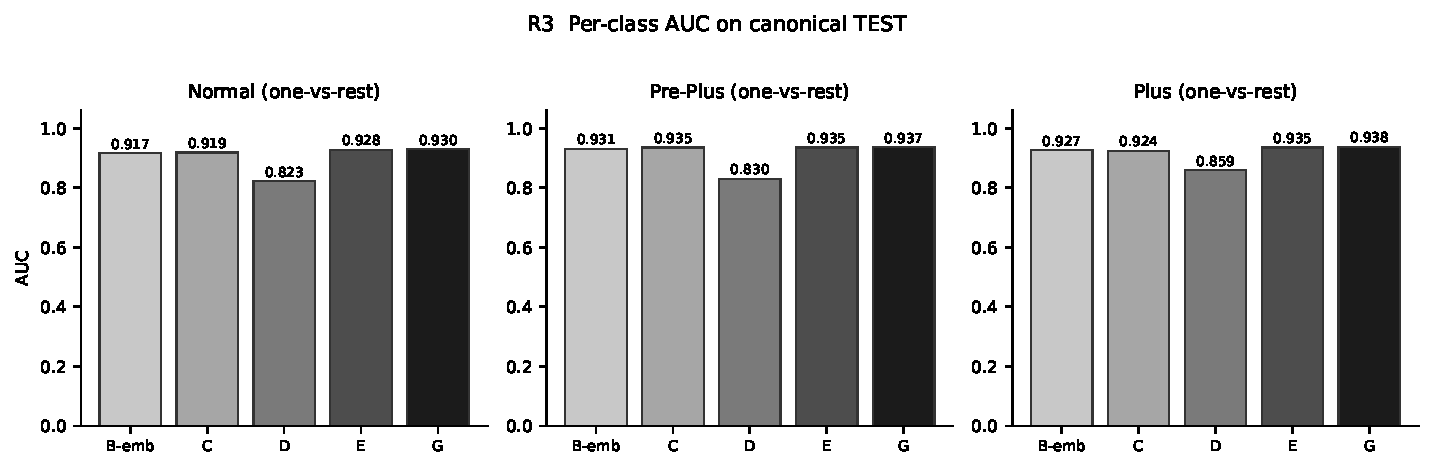
\includegraphics[width=\linewidth]{figures/main/R3_per_class_auc.pdf}
  \caption{Per-class AUC. See captions/captions\_en.md (Figure R3) for the full caption, abbreviations, statistical test, sample size and any restricted-evaluation note.}
  \label{fig:perclassauc}
\end{figure}

\begin{figure}[htbp]
  \centering
  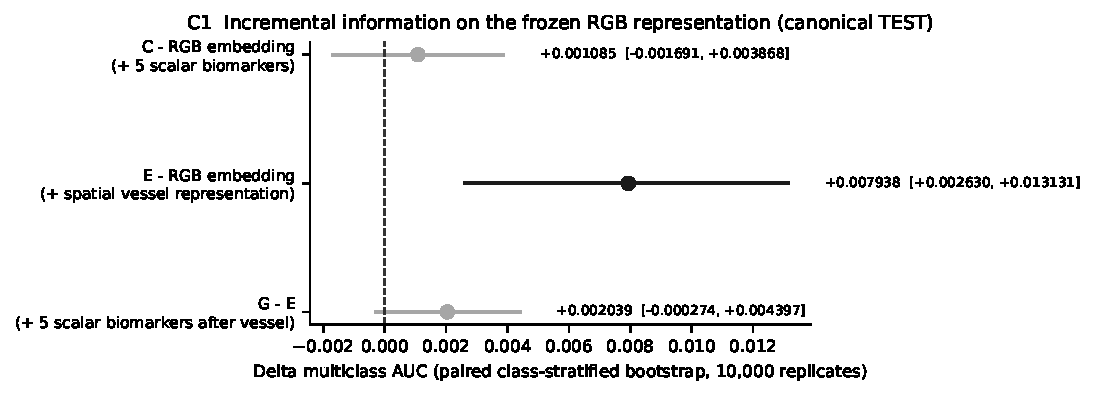
\includegraphics[width=\linewidth]{figures/main/C1_incremental_auc_forest.pdf}
  \caption{Incremental information on the frozen RGB representation. See captions/captions\_en.md (Figure C1) for the full caption, abbreviations, statistical test, sample size and any restricted-evaluation note.}
  \label{fig:incremental}
\end{figure}

\begin{figure}[htbp]
  \centering
  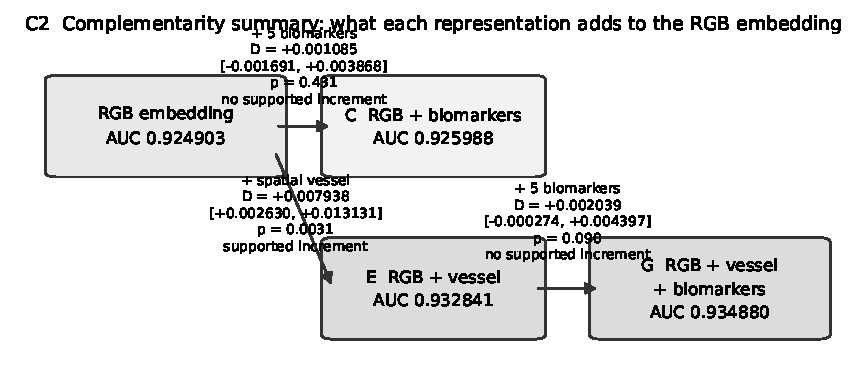
\includegraphics[width=\linewidth]{figures/main/C2_complementarity_summary.pdf}
  \caption{Complementarity summary. See captions/captions\_en.md (Figure C2) for the full caption, abbreviations, statistical test, sample size and any restricted-evaluation note.}
  \label{fig:complementarity}
\end{figure}

\begin{figure}[htbp]
  \centering
  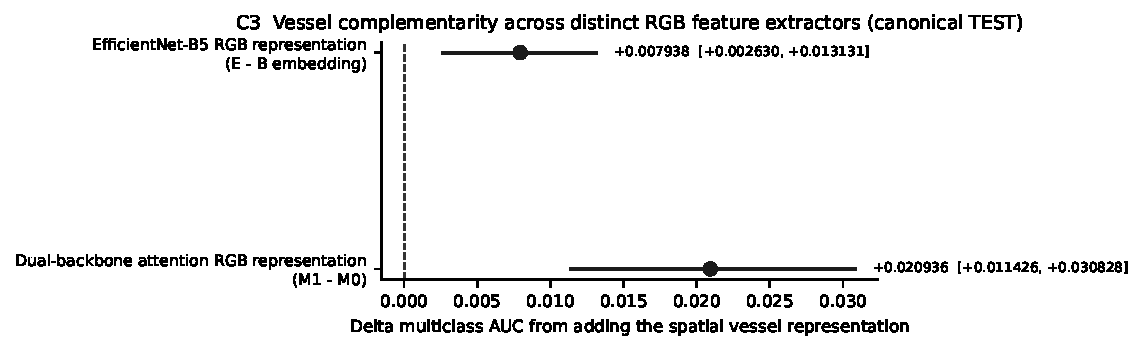
\includegraphics[width=\linewidth]{figures/main/C3_vessel_complementarity_across_rgb_architectures.pdf}
  \caption{Vessel complementarity across distinct RGB feature extractors. See captions/captions\_en.md (Figure C3) for the full caption, abbreviations, statistical test, sample size and any restricted-evaluation note.}
  \label{fig:archrobust}
\end{figure}

\begin{figure}[htbp]
  \centering
  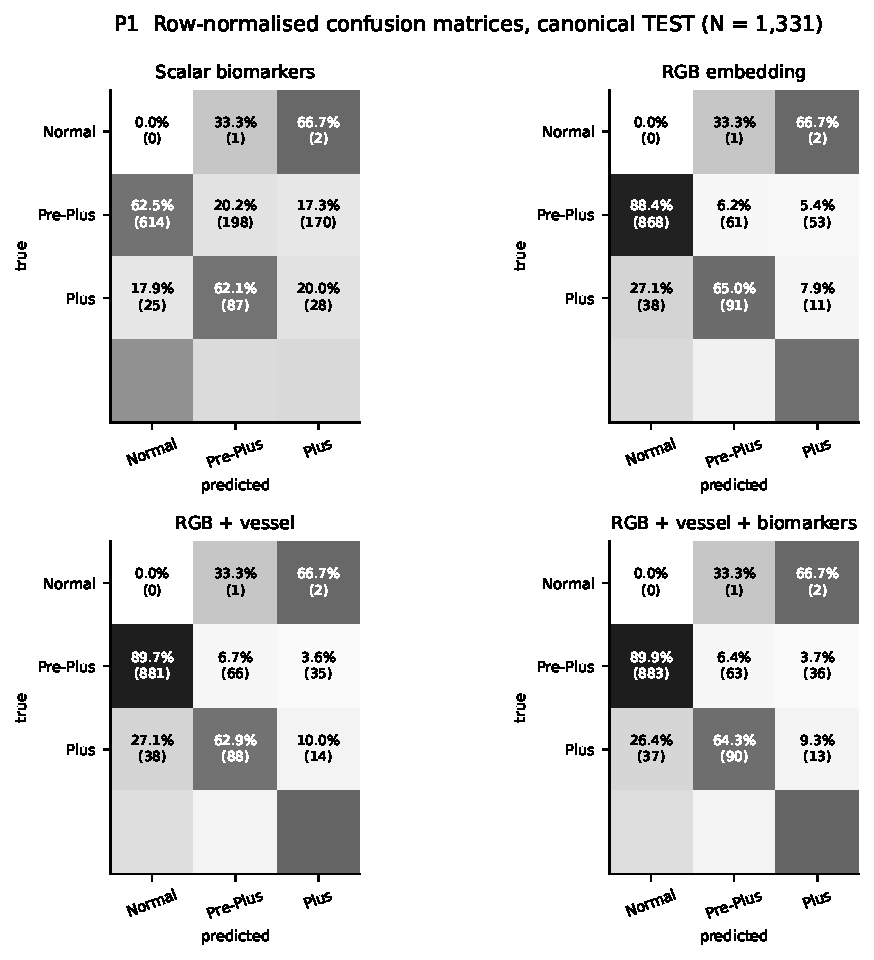
\includegraphics[width=\linewidth]{figures/main/P1_confusion_matrices_main.pdf}
  \caption{Confusion matrices. See captions/captions\_en.md (Figure P1) for the full caption, abbreviations, statistical test, sample size and any restricted-evaluation note.}
  \label{fig:confusion}
\end{figure}

\begin{figure}[htbp]
  \centering
  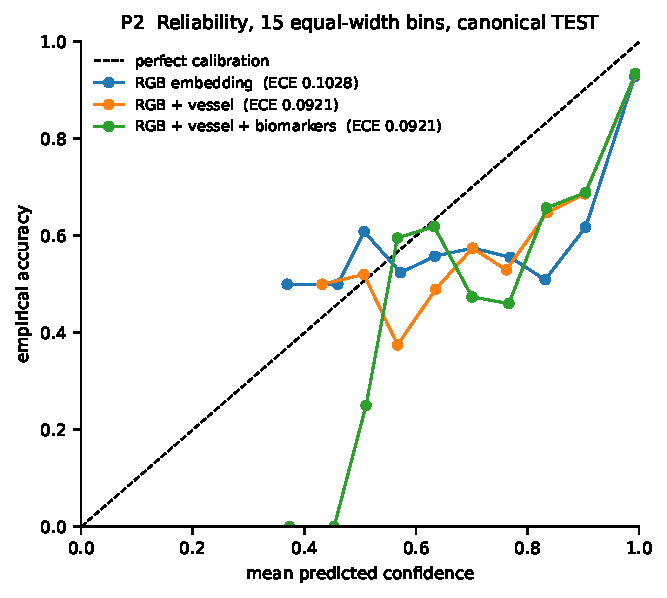
\includegraphics[width=\linewidth]{figures/main/P2_reliability_main.pdf}
  \caption{Reliability diagrams. See captions/captions\_en.md (Figure P2) for the full caption, abbreviations, statistical test, sample size and any restricted-evaluation note.}
  \label{fig:reliability}
\end{figure}

\begin{figure}[htbp]
  \centering
  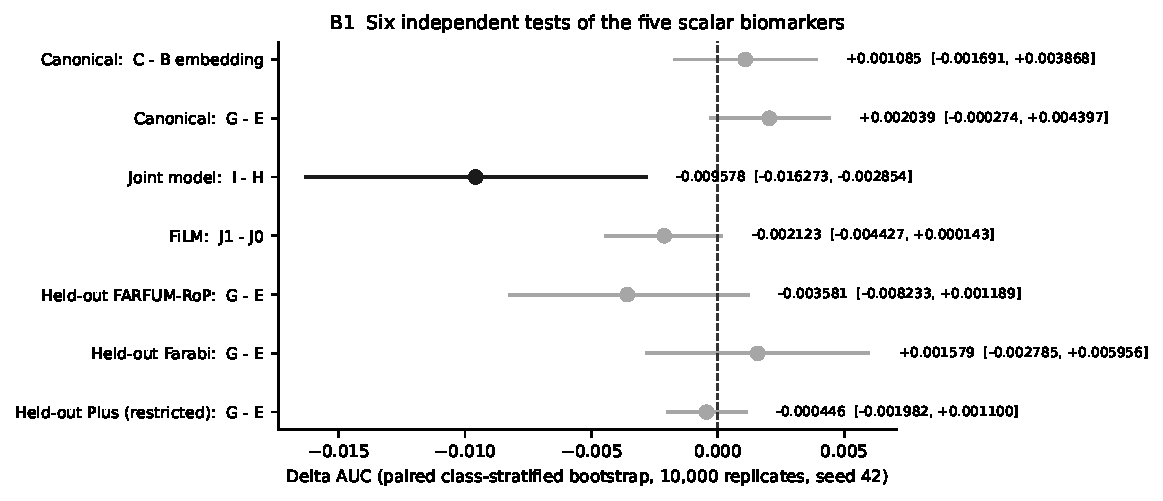
\includegraphics[width=\linewidth]{figures/main/B1_biomarker_incremental_auc_forest.pdf}
  \caption{Six independent tests of the five scalar biomarkers. See captions/captions\_en.md (Figure B1) for the full caption, abbreviations, statistical test, sample size and any restricted-evaluation note.}
  \label{fig:biomarkerforest}
\end{figure}

\begin{figure}[htbp]
  \centering
  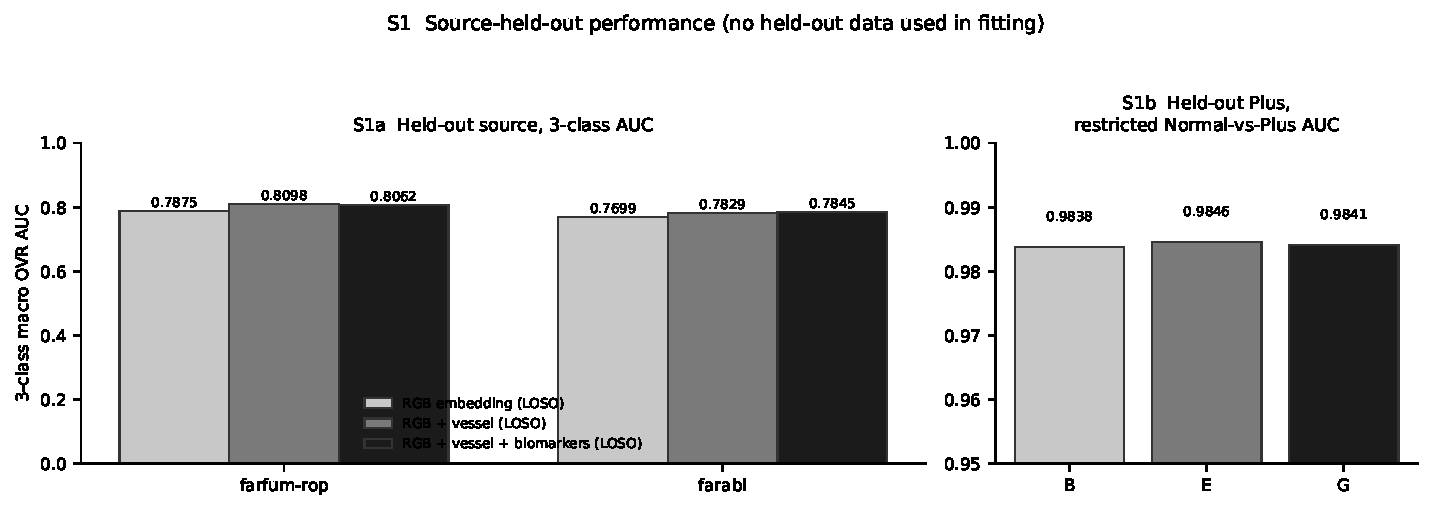
\includegraphics[width=\linewidth]{figures/main/S1_source_heldout_performance.pdf}
  \caption{Source-held-out performance. See captions/captions\_en.md (Figure S1) for the full caption, abbreviations, statistical test, sample size and any restricted-evaluation note.}
  \label{fig:loso}
\end{figure}

\begin{figure}[htbp]
  \centering
  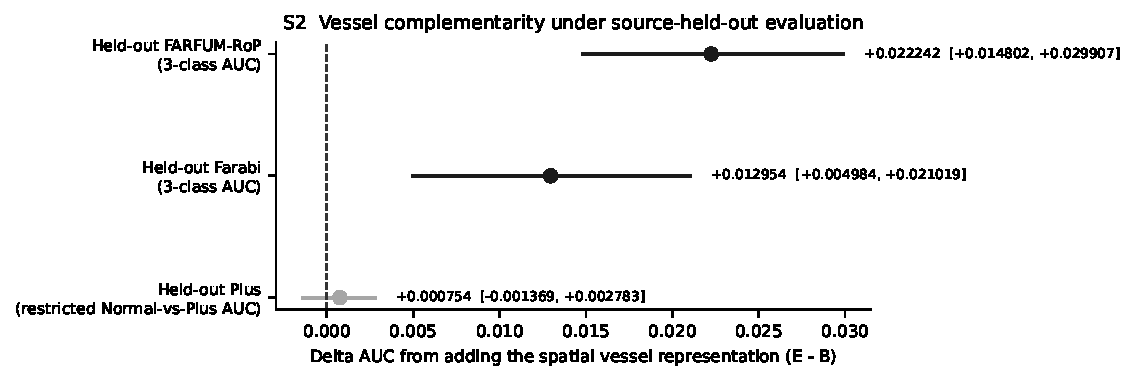
\includegraphics[width=\linewidth]{figures/main/S2_vessel_complementarity_heldout.pdf}
  \caption{Vessel complementarity under source-held-out evaluation. See captions/captions\_en.md (Figure S2) for the full caption, abbreviations, statistical test, sample size and any restricted-evaluation note.}
  \label{fig:losovessel}
\end{figure}

\begin{figure}[htbp]
  \centering
  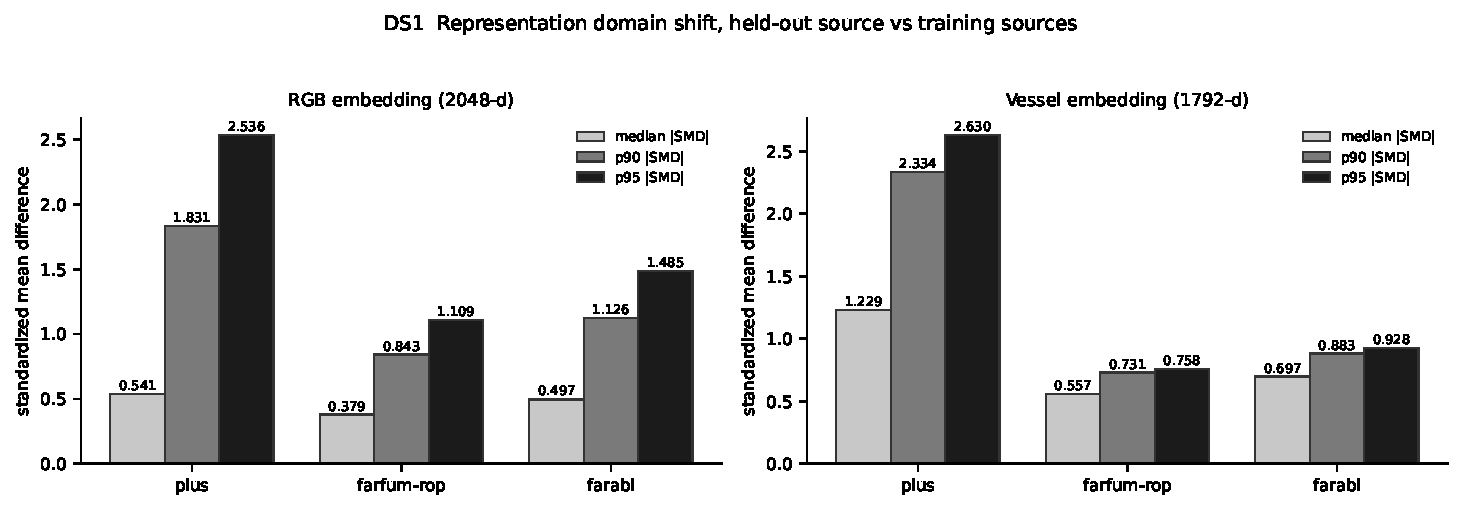
\includegraphics[width=\linewidth]{figures/main/DS1_representation_domain_shift.pdf}
  \caption{Representation domain shift. See captions/captions\_en.md (Figure DS1) for the full caption, abbreviations, statistical test, sample size and any restricted-evaluation note.}
  \label{fig:domainshift}
\end{figure}

\begin{figure}[htbp]
  \centering
  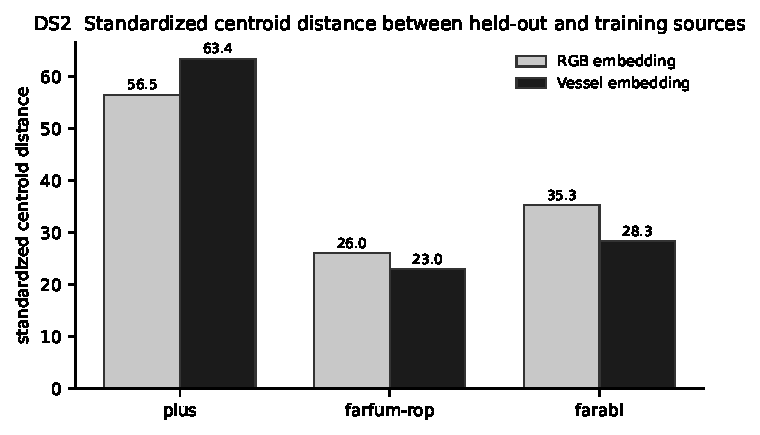
\includegraphics[width=\linewidth]{figures/main/DS2_centroid_shift.pdf}
  \caption{Standardized centroid distance. See captions/captions\_en.md (Figure DS2) for the full caption, abbreviations, statistical test, sample size and any restricted-evaluation note.}
  \label{fig:centroidshift}
\end{figure}

\begin{figure}[htbp]
  \centering
  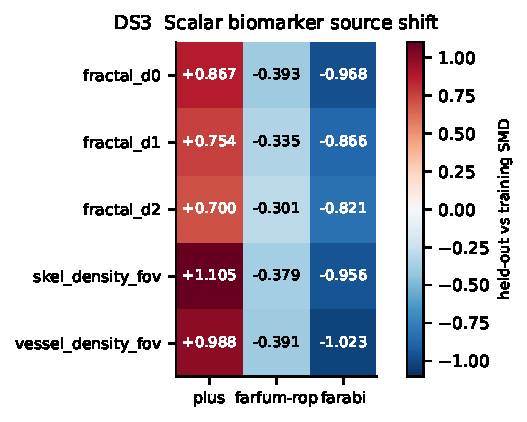
\includegraphics[width=\linewidth]{figures/main/DS3_biomarker_smd_heatmap.pdf}
  \caption{Scalar biomarker source shift. See captions/captions\_en.md (Figure DS3) for the full caption, abbreviations, statistical test, sample size and any restricted-evaluation note.}
  \label{fig:biomarkershift}
\end{figure}

\begin{figure}[htbp]
  \centering
  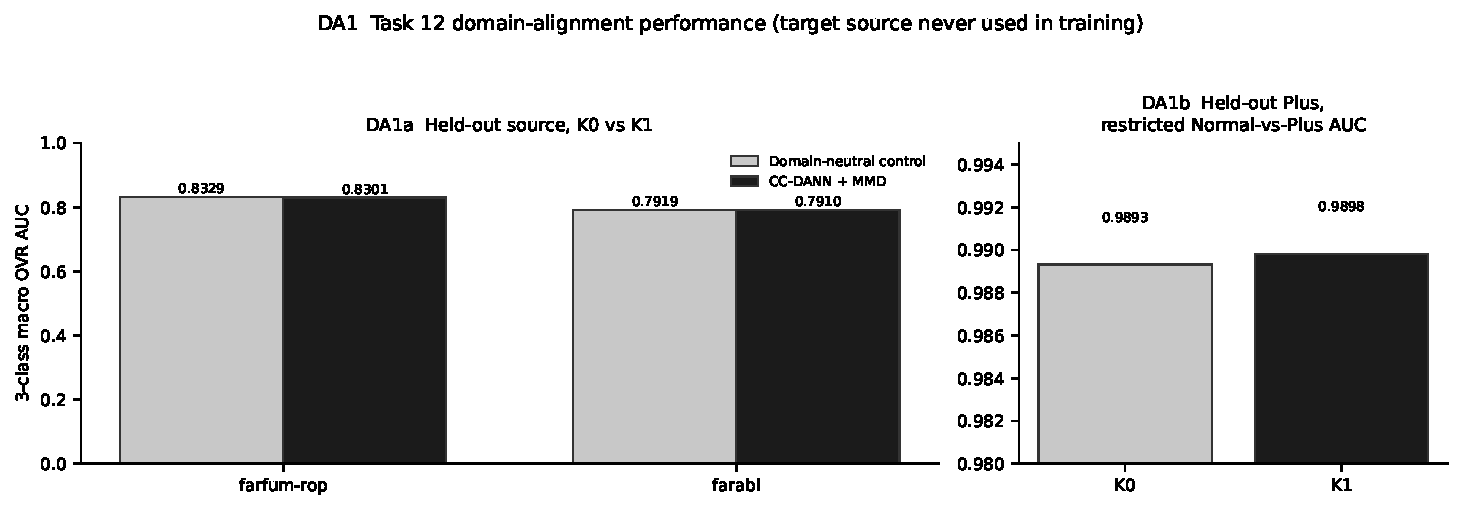
\includegraphics[width=\linewidth]{figures/main/DA1_domain_alignment_performance.pdf}
  \caption{Task 12 domain-alignment performance. See captions/captions\_en.md (Figure DA1) for the full caption, abbreviations, statistical test, sample size and any restricted-evaluation note.}
  \label{fig:daperformance}
\end{figure}

\begin{figure}[htbp]
  \centering
  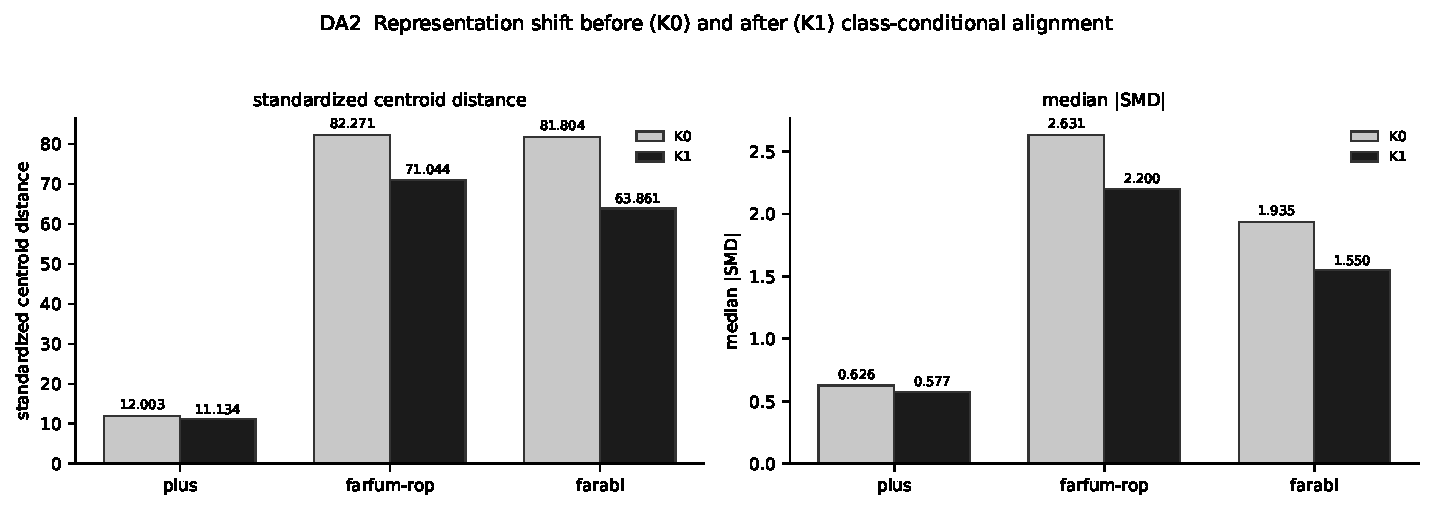
\includegraphics[width=\linewidth]{figures/main/DA2_alignment_shift_diagnostics.pdf}
  \caption{Representation shift before and after alignment. See captions/captions\_en.md (Figure DA2) for the full caption, abbreviations, statistical test, sample size and any restricted-evaluation note.}
  \label{fig:dashift}
\end{figure}

\begin{figure}[htbp]
  \centering
  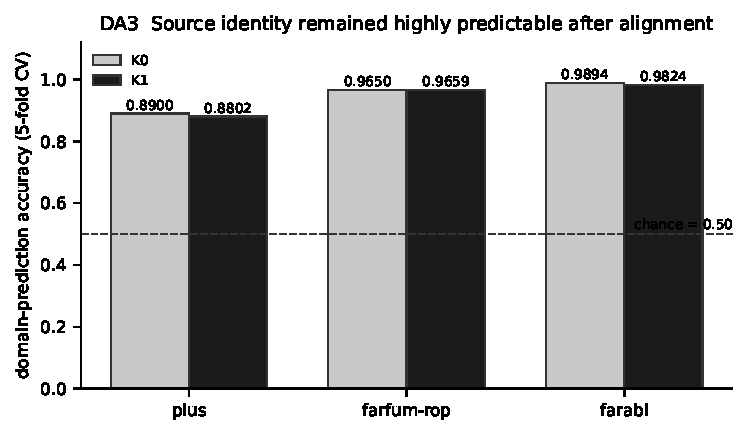
\includegraphics[width=\linewidth]{figures/main/DA3_domain_predictability.pdf}
  \caption{Domain predictability. See captions/captions\_en.md (Figure DA3) for the full caption, abbreviations, statistical test, sample size and any restricted-evaluation note.}
  \label{fig:dapredict}
\end{figure}

\begin{figure}[htbp]
  \centering
  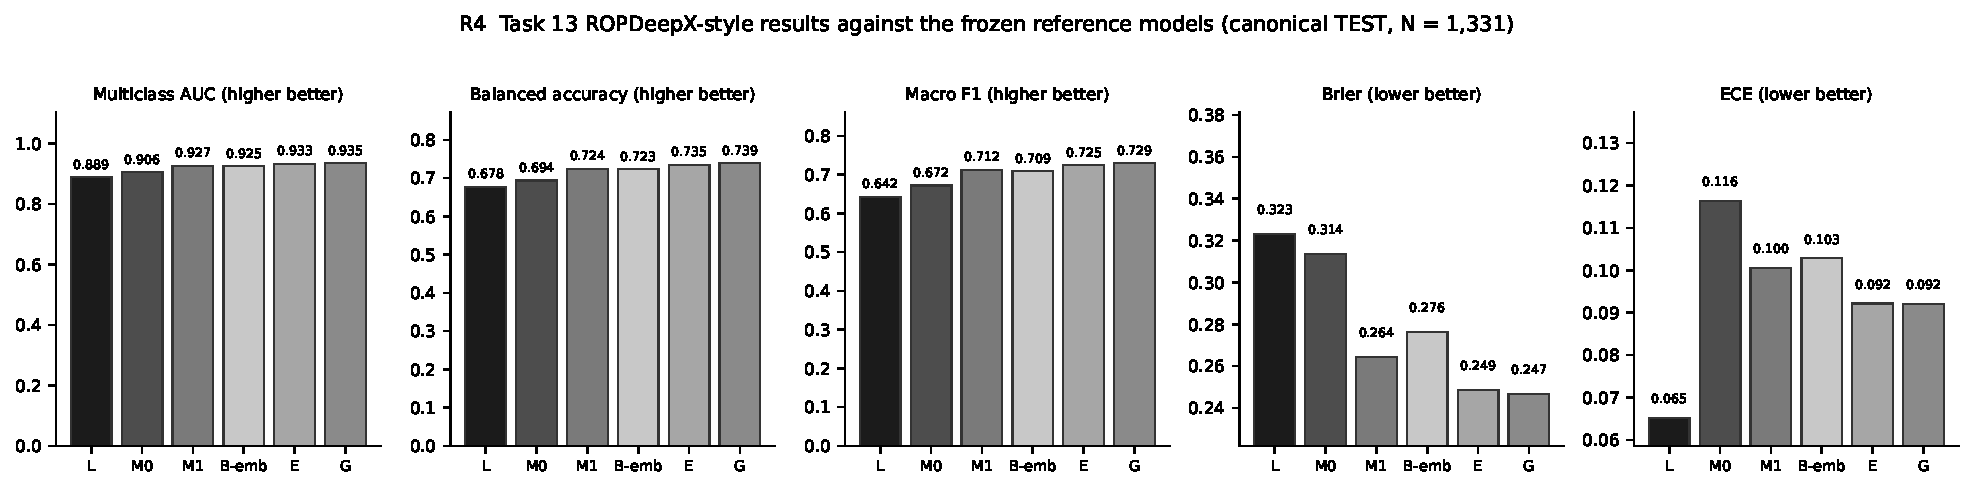
\includegraphics[width=\linewidth]{figures/main/R4_ropdeepx_style_results.pdf}
  \caption{ROPDeepX-style results. See captions/captions\_en.md (Figure R4) for the full caption, abbreviations, statistical test, sample size and any restricted-evaluation note.}
  \label{fig:ropdeepx}
\end{figure}

\begin{figure}[htbp]
  \centering
  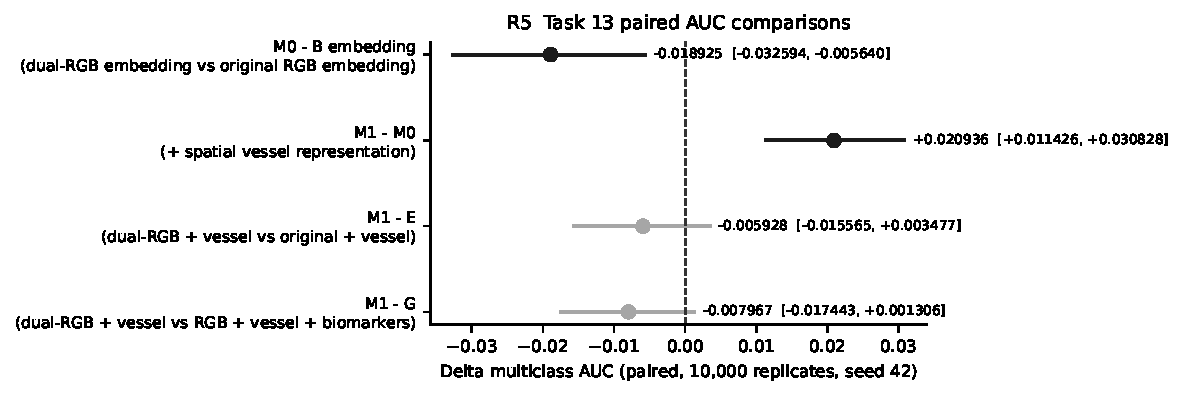
\includegraphics[width=\linewidth]{figures/main/R5_task13_paired_auc.pdf}
  \caption{Task 13 paired AUC comparisons. See captions/captions\_en.md (Figure R5) for the full caption, abbreviations, statistical test, sample size and any restricted-evaluation note.}
  \label{fig:task13paired}
\end{figure}

\begin{figure}[htbp]
  \centering
  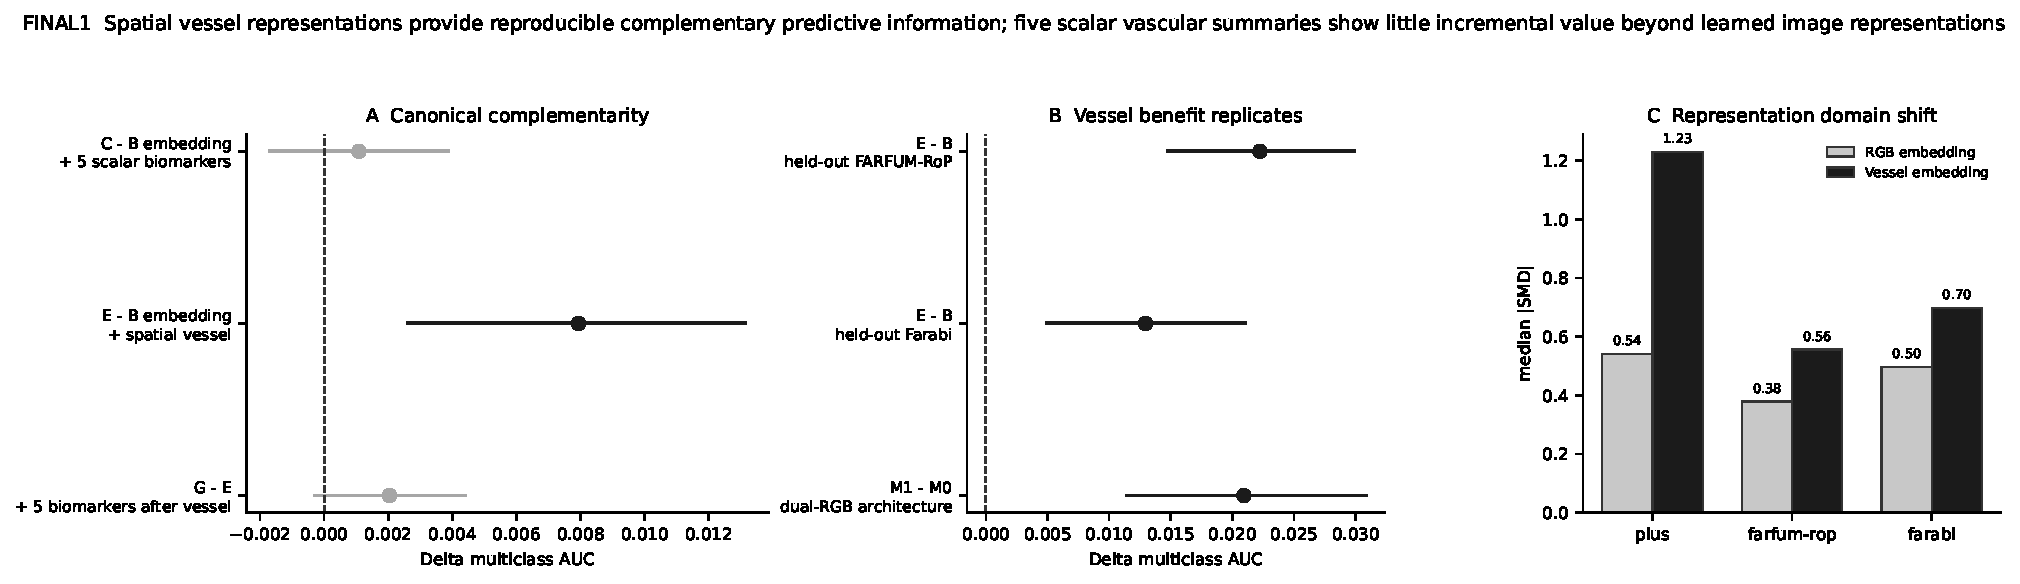
\includegraphics[width=\linewidth]{figures/main/FINAL1_thesis_summary.pdf}
  \caption{Thesis summary. See captions/captions\_en.md (Figure FINAL1) for the full caption, abbreviations, statistical test, sample size and any restricted-evaluation note.}
  \label{fig:summary}
\end{figure}

\begin{figure}[htbp]
  \centering
  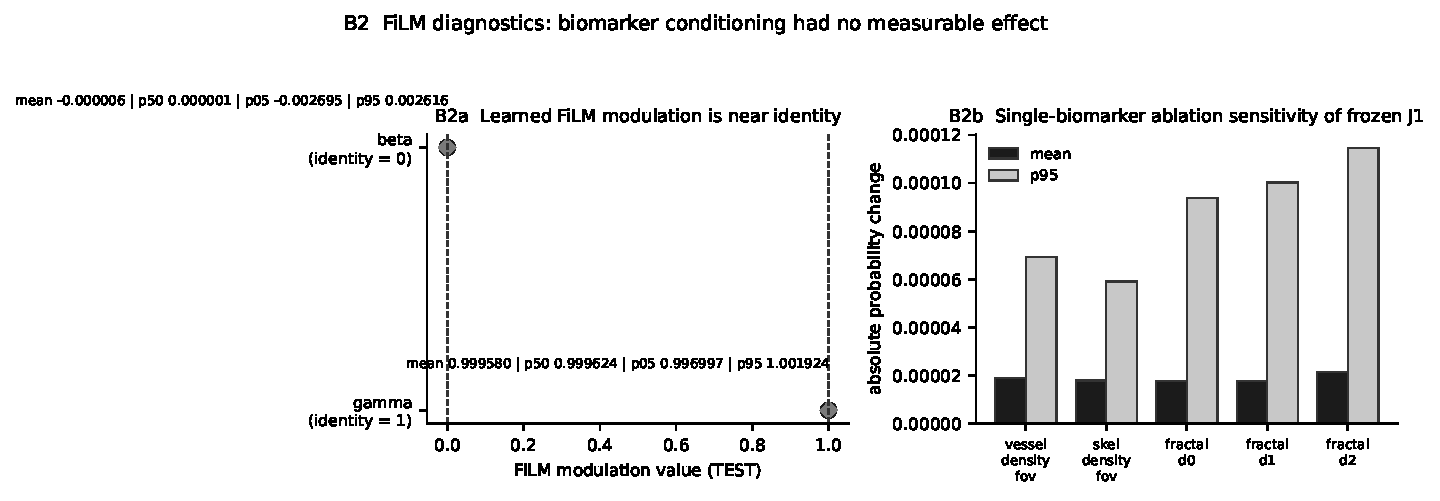
\includegraphics[width=\linewidth]{figures/appendix/B2_film_diagnostics.pdf}
  \caption{FiLM diagnostics. See captions/captions\_en.md (Figure B2) for the full caption, abbreviations, statistical test, sample size and any restricted-evaluation note.}
  \label{fig:film}
\end{figure}

\begin{figure}[htbp]
  \centering
  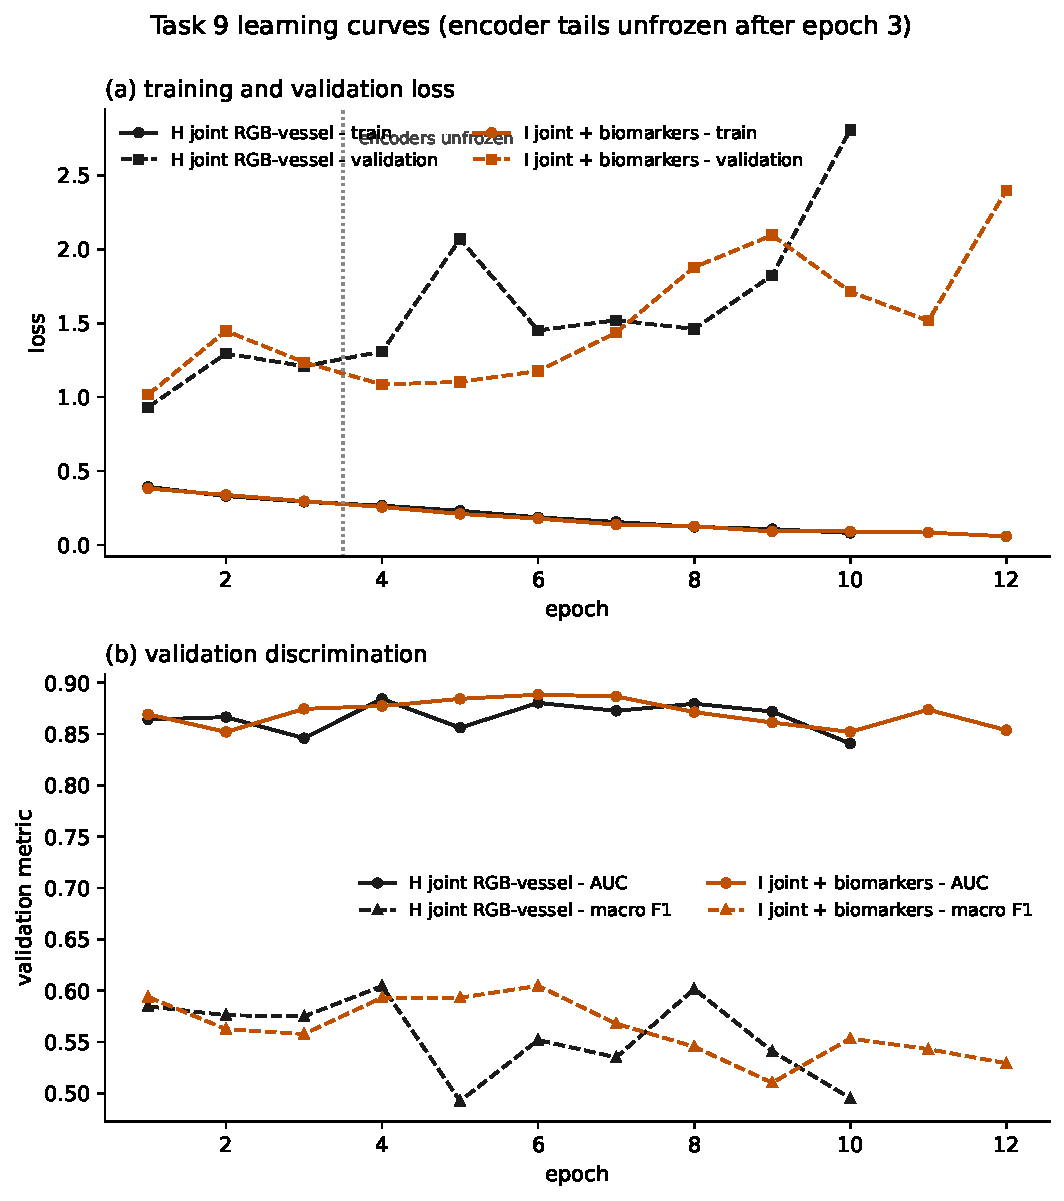
\includegraphics[width=\linewidth]{figures/appendix/N1_task9_learning_curves.pdf}
  \caption{Task 9 learning curves. See captions/captions\_en.md (Figure N1) for the full caption, abbreviations, statistical test, sample size and any restricted-evaluation note.}
  \label{fig:n1}
\end{figure}

\begin{figure}[htbp]
  \centering
  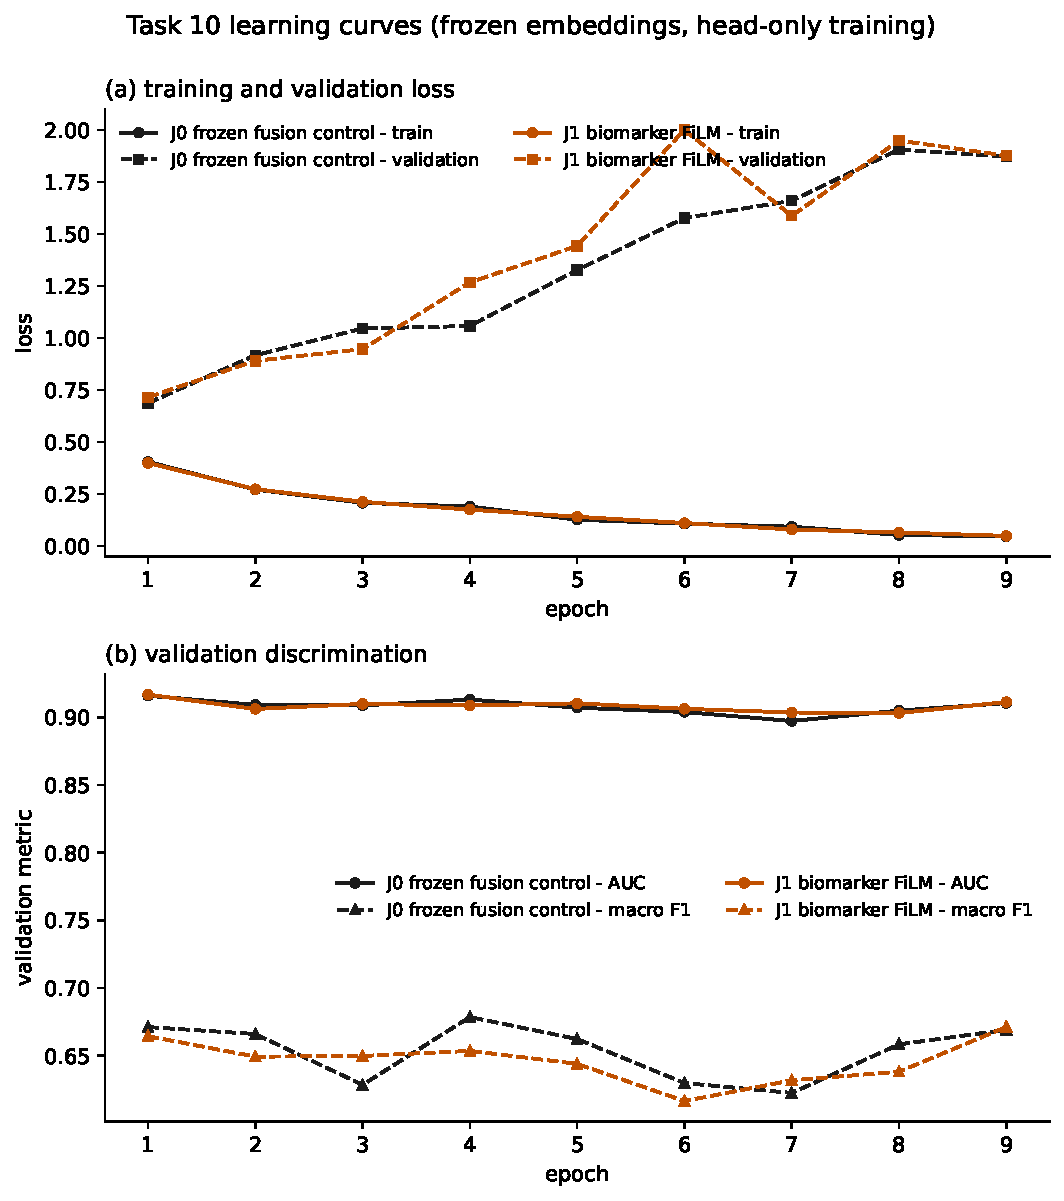
\includegraphics[width=\linewidth]{figures/appendix/N2_task10_learning_curves.pdf}
  \caption{Task 10 learning curves. See captions/captions\_en.md (Figure N2) for the full caption, abbreviations, statistical test, sample size and any restricted-evaluation note.}
  \label{fig:n2}
\end{figure}

\begin{figure}[htbp]
  \centering
  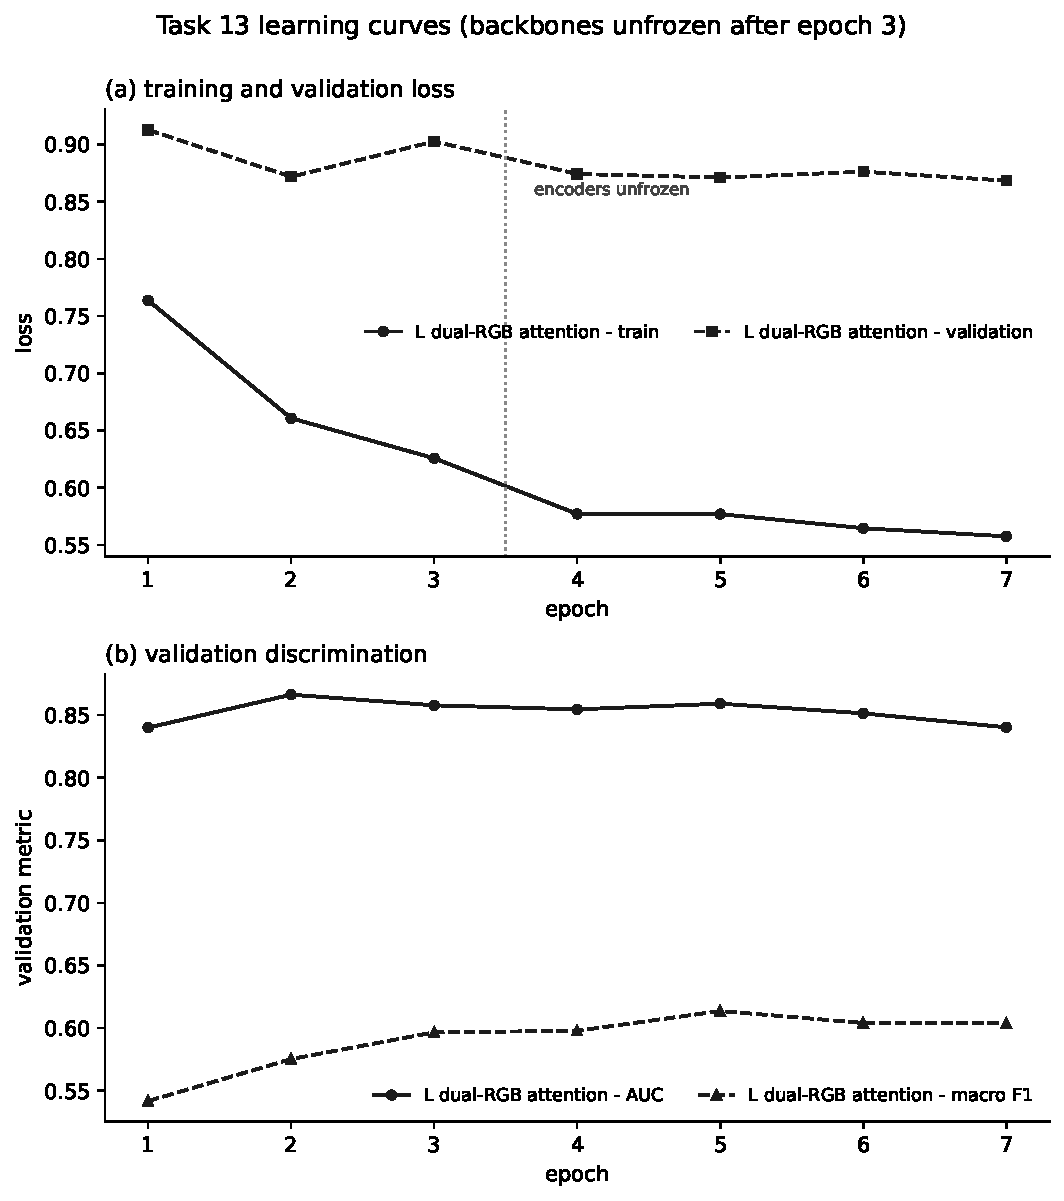
\includegraphics[width=\linewidth]{figures/appendix/N3_task13_learning_curves.pdf}
  \caption{Task 13 learning curves. See captions/captions\_en.md (Figure N3) for the full caption, abbreviations, statistical test, sample size and any restricted-evaluation note.}
  \label{fig:n3}
\end{figure}

\begin{figure}[htbp]
  \centering
  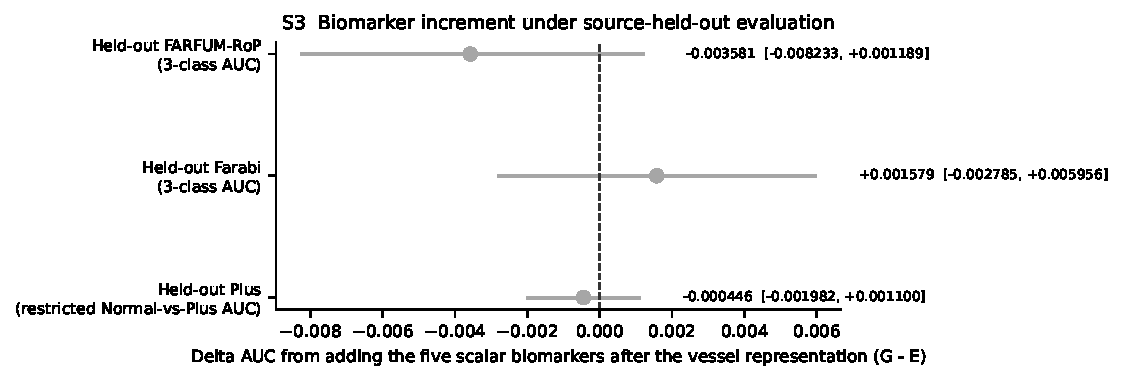
\includegraphics[width=\linewidth]{figures/appendix/S3_biomarker_heldout_forest.pdf}
  \caption{Biomarker increment under source-held-out evaluation. See captions/captions\_en.md (Figure S3) for the full caption, abbreviations, statistical test, sample size and any restricted-evaluation note.}
  \label{fig:s3}
\end{figure}

\begin{figure}[htbp]
  \centering
  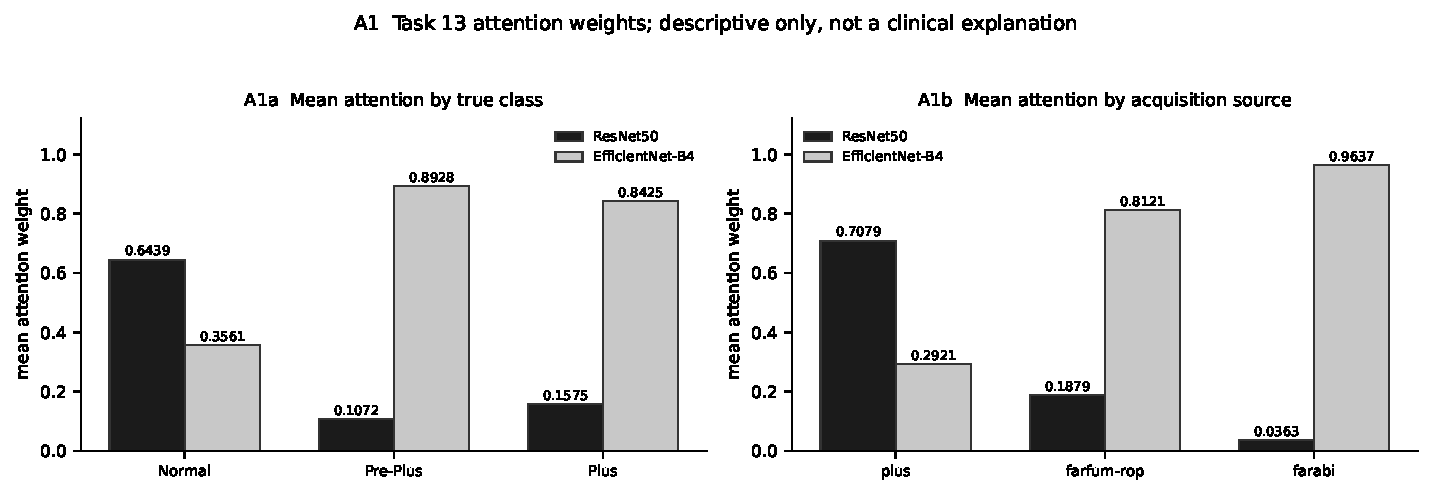
\includegraphics[width=\linewidth]{figures/appendix/A1_attention_by_class_and_source.pdf}
  \caption{Attention weights by class and source. See captions/captions\_en.md (Figure A1) for the full caption, abbreviations, statistical test, sample size and any restricted-evaluation note.}
  \label{fig:a1}
\end{figure}

\begin{figure}[htbp]
  \centering
  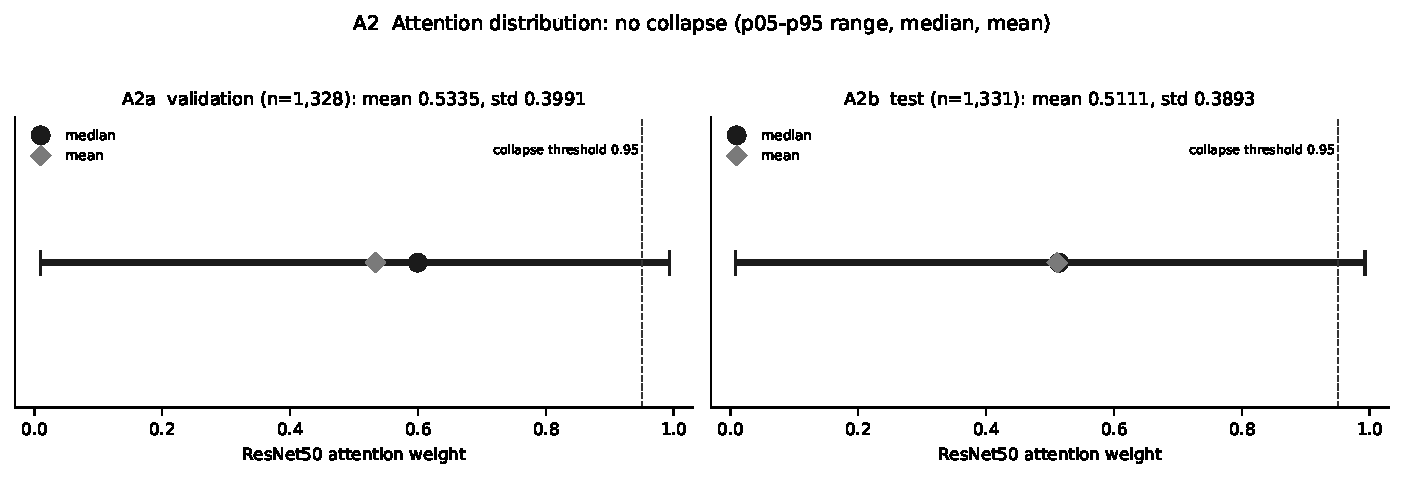
\includegraphics[width=\linewidth]{figures/appendix/A2_attention_distribution.pdf}
  \caption{Attention distribution. See captions/captions\_en.md (Figure A2) for the full caption, abbreviations, statistical test, sample size and any restricted-evaluation note.}
  \label{fig:a2}
\end{figure}
